% 103-15(103쪽) — 원점을 출발한 점 P 의 시각 t 에서의 위치 x(t) 의 그래프(t=1 에서 극대 1, t=2 에서 극소 -1, t=5 에서 극대 2, t=3·6 에서 0). 스캔 화질이 낮아 TikZ 로 다시 그림.
% 원문에 있는 것만 옮긴다: 곡선 · 안내 점선(1, 2, 4, 5) · 눈금 2, 1, -1 · 라벨 x(t), t, O, 1, 2, 3, 4, 5, 6.
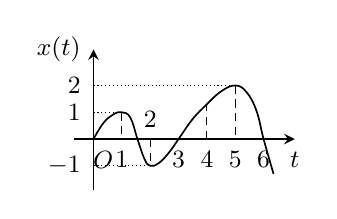
\begin{tikzpicture}[x=0.36cm, y=0.34cm, line width=0.6pt]
  \draw[->, >=stealth, line width=0.7pt] (-0.7,0) -- (7.1,0) node[below=1pt, font=\small] {$t$};
  \draw[->, >=stealth, line width=0.7pt] (0,-1.90) -- (0,3.35) node[left=1pt, font=\small] {$x(t)$};
  \draw[densely dotted, line width=0.4pt] (0,1) -- (1,1);
  \draw[densely dashed, line width=0.4pt] (1,1) -- (1,0);
  \draw[densely dotted, line width=0.4pt] (0,-1) -- (2,-1);
  \draw[densely dashed, line width=0.4pt] (2,0) -- (2,-1);
  \draw[densely dashed, line width=0.4pt] (4,0) -- (4,1.30);
  \draw[densely dotted, line width=0.4pt] (0,2) -- (5,2);
  \draw[densely dashed, line width=0.4pt] (5,2) -- (5,0);
  \draw plot[smooth, tension=0.7] coordinates {(0,0) (0.35,0.60) (0.70,0.92) (1,1) (1.30,0.80) (1.55,0) (1.80,-0.75) (2,-1) (2.30,-0.90) (2.65,-0.52) (3,0) (3.50,0.75) (4,1.30) (4.50,1.78) (5,2) (5.40,1.75) (5.75,1.05) (6,0) (6.35,-1.30)};
  \node[below=1pt, font=\small] at (0.34,0) {$\pt{O}$};
  \node[below=1pt, font=\small] at (1,0) {$1$};
  \node[above=0.5pt, font=\small] at (2,0) {$2$};
  \node[below=1pt, font=\small] at (3,0) {$3$};
  \node[below=1pt, font=\small] at (4,0) {$4$};
  \node[below=1pt, font=\small] at (5,0) {$5$};
  \node[below=1pt, font=\small] at (6,0) {$6$};
  \node[left=1pt, font=\small] at (0,1) {$1$};
  \node[left=1pt, font=\small] at (0,2) {$2$};
  \node[left=1pt, font=\small] at (0,-1) {$-1$};
\end{tikzpicture}
